\chapter{ทฤษฎีความรู้และงานที่เกี่ยวข้อง}

\emph{หัวข้อต่าง ๆ ในแต่ละบทเป็นเพียงตัวอย่างเท่านั้น หัวข้อที่จะใส่ในแต่ละบทขึ้นอยู่กับโปรเจคของนักศึกษาและอาจารย์ที่ปรึกษา}

ตัวอย่างการใส่อ้างอิงที่มา -> \cite{hypersense} ถ้าต้องการใส่แหล่งอ้างอิงมากกว่า 1 ให้ทำดังนี้ -> \cite{hypersense,bworld}
อธิบายทฤษฎี องค์ความรู้หลักที่ใช้ในงาน งานวิจัยที่นำมาใช้ในโครงงาน หรือเปรียบเทียบผลิตภัณฑ์ที่มีอยู่ในท้องตลาด\cite{bworld}
Explain theory, algorithms, protocols, or existing research works and tools related to your work.


\section{ระบบแนะนำสินค้า}

\begin{table}[!h]
    \caption{test table method1}\label{tbl:method1}
    \begin{tabular}{c|c|l|rr} \hline\hline
        Center & Center & left aligned & Right & Right aligned \\ \hline\hline
        Center & Center & left aligned & Right & Right aligned \\ \hline
        Center & Center & left aligned & Right & Right aligned \\
        Center & Center & left aligned & Right & Right aligned \\ \hline
        Center & Center & left aligned & Right & Right aligned \\ \hline\hline
    \end{tabular}
\end{table}


\section{อัลกอริทึมในการประมวลผลข้อความ}
\subsection{อัลกอริทึม I}

% Can define this in the preamble..
You can place the figure and refer to it as รูปที่~\ref{fig:model2}.
The figure and table numbering will be run and updated automatically when you add/remove tables/figures from the document.

\begin{figure}[!h]\centering
    \setlength{\fboxrule}{0.2mm} % can define this in the preamble
    \setlength{\fboxsep}{1cm}
    \fbox{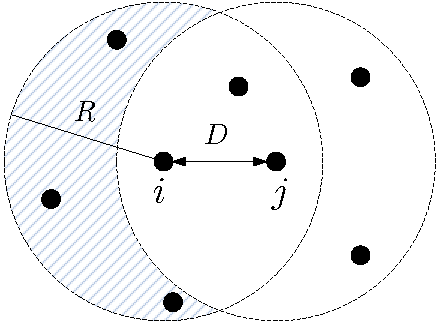
\includegraphics[width=5cm]{./model2.pdf}}
    \caption{The network model}\label{fig:model2}
\end{figure}


\subsection{อัลกอริทึม II}
Add more subsections as you want.
\subsubsection{ขั้นตอนที่ 1}
\subsubsection{ขั้นตอนที่ 2}
Latex Format นี้รองรับหัวข้อย่อยถึงแค่ระดับ 4 นี้เท่านั้น ไม่แนะนำให้แบ่งหัวข้อย่อยไปมากกว่านี้ เช่น 2.2.2.2.1 , 2.2.2.2.2

\section{เครื่องมือที่ใช้ในการพัฒนา}